\documentclass{beamer}




\usepackage[T1,T2A]{fontenc}
\usepackage[utf8]{inputenc}

\usepackage{graphicx}
\usepackage{blindtext}
\usepackage{ mathrsfs }
\usepackage[russian,english]{babel}
%\usepackage{ dsfont }

\author{Деркач Максим Юрьевич}
\title{Криптографические протоколы}
\subtitle{Протоколы WEP, WPA, WPA2, WPA3}
\setbeamercolor{frametitle}{bg=cyan!10}


%\usetheme{lucid}
\begin{document}
	\frame {
		\titlepage
	}
	\frame {
		\frametitle{Ссылки}
		
		\url{https://www.cs.jhu.edu/~Eastubble/dss/ae.pdf}
		\url{http://cseweb.ucsd.edu/~mihir/papers/oem.pdf}
		\url{https://habr.com/en/post/425637/}
				
			
	}
	\frame{
		\frametitle{Введение}
		\textbf{WEP (Wired Equivalent Privacy)} - один из старейших протоколов безопасности, который может использовать WiFi-маршрутизатор, и он не очень безопасный. Он был использован в 1990-х годах, но с тех пор были разработаны другие протоколы безопасности.
		
		\textbf{WPA (Wi-Fi Protected Access)} - это протокол, который первоначально заменило WEP как более безопасный способ хранения данных. В то время он был не идеален, но он лучше, чем WEP. Весь смысл разработки этого протокола состоял в том, чтобы преодолеть некоторые из основных недостатков WEP.
	}

	\frame{
	\frametitle{WEP}

В основе WEP лежит поточный шифр \textbf{RC4}, выбранный из-за своей высокой скорости работы и возможности использования переменной длины ключа. Для подсчета контрольных сумм используется \textbf{CRC32}. 

\bigskip


}

\bigskip
	\frame{
	\frametitle{WEP}
	
	Пакет WEP протокола состоит из 2 частей:
	\begin{enumerate}
		\item Открытые данные:
		\begin{enumerate}
			\item Синхропосылка (IV) - 3 байта;
			\item Пустое место (Padding) - 6 бит;
			\item Идентификатор ключа (Key ID) - 2 бит;
		\end{enumerate}
		\item Зашифрованные данные:
		\begin{enumerate}
			\item Данные
			\item Контрольная сумма
		\end{enumerate}
	\end{enumerate}
	
	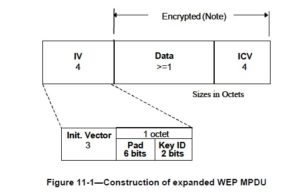
\includegraphics[width=0.8\linewidth]{wep_packet.jpg}
}

	\frame{
	\frametitle{WEP Auth Protocol}
		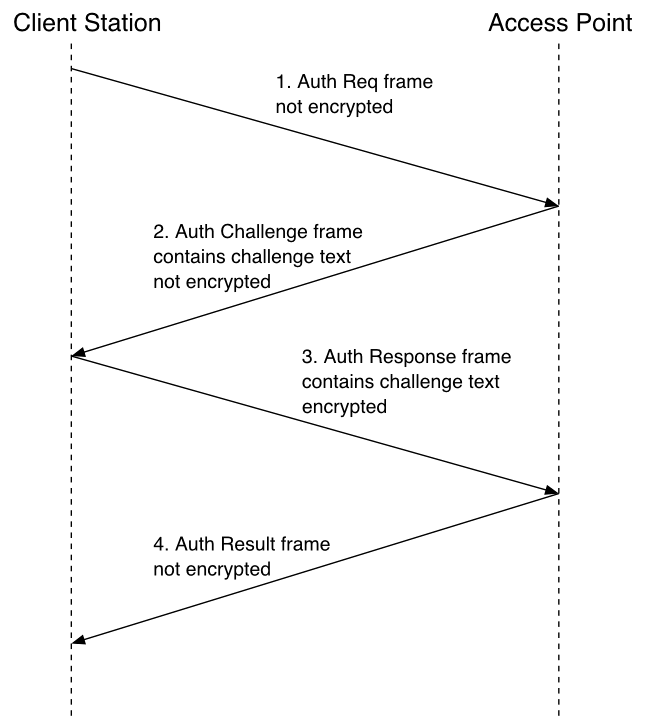
\includegraphics[width=0.7\linewidth]{wep_protocol.png}
}

\frame{
	\frametitle{WEP Encryption and Decryption}
		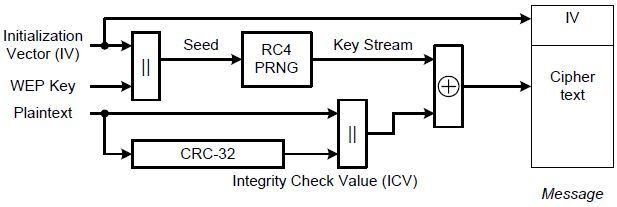
\includegraphics[width=0.8\linewidth]{wep_encap.png}
		
		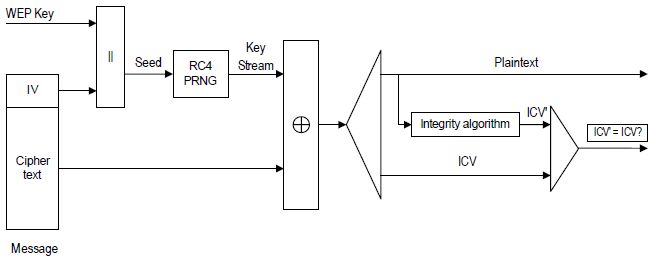
\includegraphics[width=0.8\linewidth]{wep_decap.png}
}

\frame{
	\frametitle{WEP Security}
	В протоколе WEP есть множество слабых мест:
	\begin{enumerate}
		\item механизмы обмена ключами и проверки целостности данных:
		\begin{itemize}
		\item В качестве MAC функции в WEP используется некриптографический алгоритм CRC.
		\end{itemize}	
		\item малая разрядность ключа и вектора инициализации:
		\begin{itemize}
		\item Повторное использование IV создает идентичные ключевые потоки, и поскольку длина IV мала, это гарантирует, что IV повторится через относительно короткое время (5-7 часов) в загруженной сети.
		\item Стандарт 802.11 не описывал ограничения и правила на генерацию IV. Поэтому некоторые производители беспроводных адаптеров генерировали одинаковые последовательности IV, постоянное IV. В результате хакеры могли записывать сетевой трафик, определять поток ключей и использовать его для расшифровки зашифрованного текста.
		\end{itemize}
		\item способ аутентификации;
		\item алгоритм шифрования.
	\end{enumerate}

}

	\frame {
	\begin{figure}
		%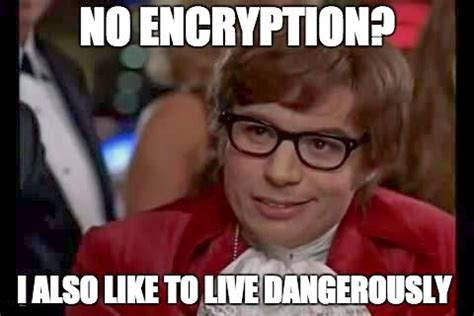
\includegraphics[width=0.8\linewidth]{memes1.jpeg}
		
	\end{figure}
	}

\end{document}